\section{Methods}

The code for the project is available at  \cite{project_repo}.

\subsection{Acquiring the datasets}

We primarily work with a dataset of geolocated Swiss tweets provided by the ADA team (originally by Swisscom). The tweets were queried using a bounding box around Switzerland, which means that not all tweets are actually Swiss. We will explain how we filter the ones outside of Switzerland in section \ref{pre_geo}.

We also used several supporting datasets, which were not straightforward to locate and acquire. The geojson file for the boundary of Swiss municipalities was downloaded from \cite{swiss_geo}. The population data was acquired from \cite{pop_data} and the population densities were downloaded from \cite{swiss_pop_density}. For detecting political activity we used the data of \cite{tw_useful} available at \cite{swiss_political_users}.
\subsection{Preprocessing data}

\subsubsection{Reading the data}

Parsing the provided dataset was in itself a demanding challenge, so we decided to dedicate a subsection to it. The data was provided in the tab separated values format; columns were separated by \textbackslash t and rows by \textbackslash n. However, many of the tweets contained tabs and newlines, these were denoted by \textbackslash\textbackslash t and \textbackslash\textbackslash n. To make it more complicated the last column (userLocation) sometimes ended with a large number of backslashes which resulted in further ambiguity. Since even after resolving all these exceptions and a few others, we still got rows with varying  length, we decided to follow a different approach.

The first three columns of the dataset (id, userid, createdAt (date)) were all not nullable and very robust in terms of syntax. We decided to match a regular expression on


\begin{Verbatim}[frame=single,fontsize=\scriptsize]
  \d{4,}\t\d{4,}\t\d{4}\-\d{2}\-\d{2}\s\d{2}:\d{2}:\d{2}
\end{Verbatim}

which proved to be very reliable in our tests. This allowed us to find the beginning of each row, however, separating the cells was still difficult. We decided to split on \textbackslash t, and merge together the cells [3:-16] as the text cell, since we expected that the last 16 and the first 3 columns had no \textbackslash t, only possibly $4^{th}$ (text) column. It turned out that we were wrong, the last ($20^{th}$) column (userLocation) also had \textbackslash t, but these exceptions only involved less than 20000 datapoints (out of $\sim$ 20 million), so we neglected these. We will see later that this is a tiny fraction compared to the fraction of datapoints we had to exclude due to other issues with the dataset.

\subsubsection{Processing geolocation}
\label{pre_geo}

Out of the $\sim$ 20 million tweets, about $\sim$ 18 million were geolocated. Only about 10 million these geolocations were in Switzerland (the rest came from neighbouring countries in the bounding box). Since our goal was to analyse only Swiss tweets, the rest of the datapoints (about 50\% of the whole) had to be dropped.

For our later analyses, we had to detect the municipality each tweet came from. We made use of the geojson map which contained the boundaries of each  municipality as a polygon, and we used the \textit{shapely} python library to detect which polygon each geolocation is in \cite{shapely}. Since the 10 million tweets came from only less than 15000 unique locations (probably since the geolocations were not the exact locations of the users, rather maybe the location of the transmissing tower each cellphone was connected to), we could compute the municipality information in less than 30 minutes.

\begin{figure}[h]
  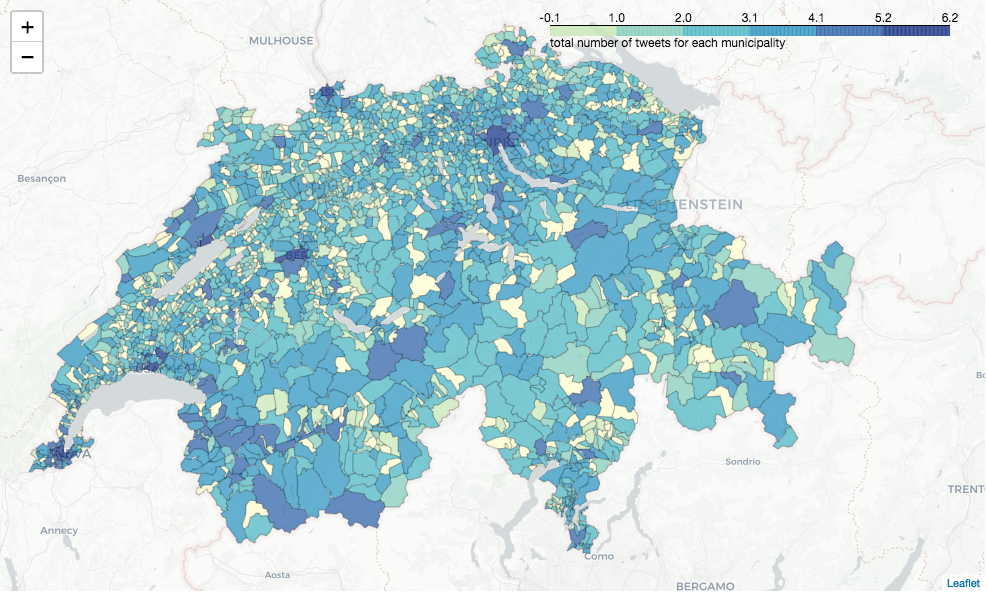
\includegraphics[width=0.5\textwidth]{images/all_tweet_map.png}
  \caption{Colors on the map show the logarithm (base 10) of the number of tweets in the whole dataset coming from each municipality}
  \label{all_tweet_map}
\end{figure}


\begin{figure}[h]
  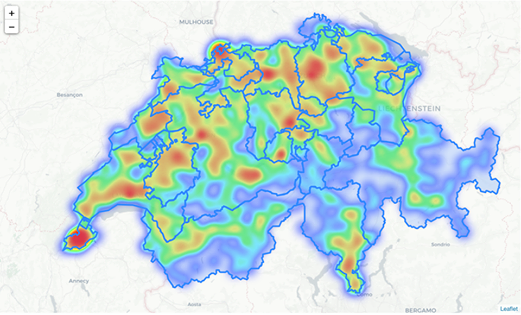
\includegraphics[width=0.5\textwidth]{images/heat_map.png}
  \caption{The heatmap of the number of tweets in September 2016.}
  \label{heat_map}
\end{figure}



\subsubsection{Language detection}

Language detection was a crucial step especially for research question 2, but also for detecting political content. For this task, we used the \textit{langdetect} python library \cite{pylangdetect}, a port of Google's language detection code based on a naive Bayesian filter \cite{nakatani2010langdetect}. This is the only task for which we had to use the hadoop cluster. Our simple spark code took 3 hours on 50 nodes.

Unfortunately, by manual inspection we saw that the accuracy of \textit{langdetect} was far from perfect (even though the website claimed 99\% accuracy). One of our concerns was that possibly the Swiss German dialect could cause problems, so we downloaded a Swiss German corpus and tested \textit{langdetect} on the sentences of the text. On the collection of Swiss German blogposts we saw an accuracy above 82\%, whereas on the ``Blick am Abig" newspaper from Z\"urich our accuracy was above 95\% (the majority of tweets were classified as simply german in both cases). After this confirmation, we concluded that the observed errors are probably due to the fact that tweets are short and don't follow the rules of the languages very closely. 

The distribution of tweets over the municipalities is visualized on Figure \ref{all_tweet_map}. On Figure \ref{heat_map} we show a heatmap of twitter activity for only one month (over the whole dataset this was too computation intensive).

\begin{figure}[h]
  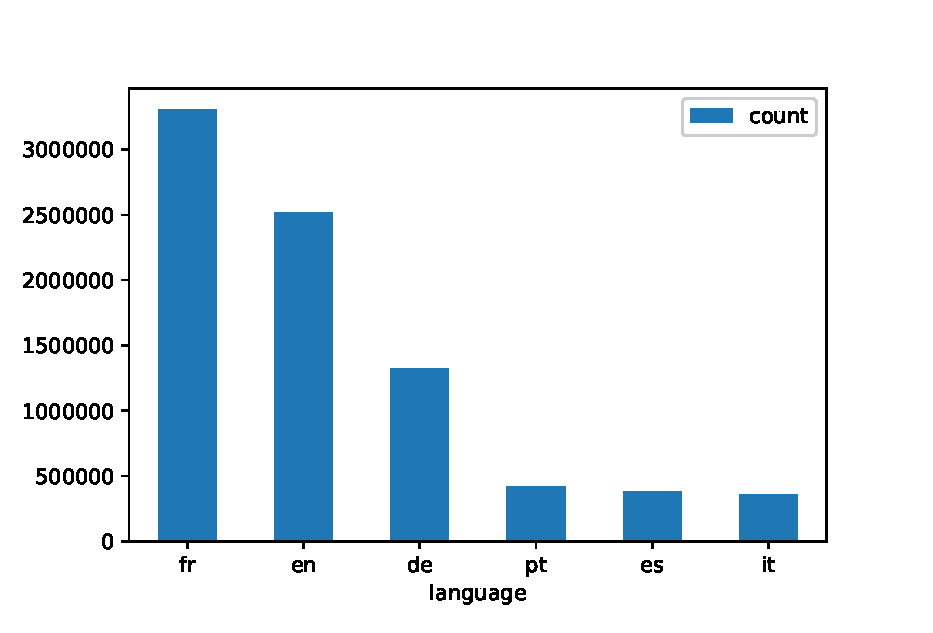
\includegraphics[width=0.45\textwidth]{images/swiss_counts.eps}
  \caption{The number of tweets in the top5 languages in the dataset}
  \label{swiss_counts}
\end{figure}



\begin{figure}[h]
  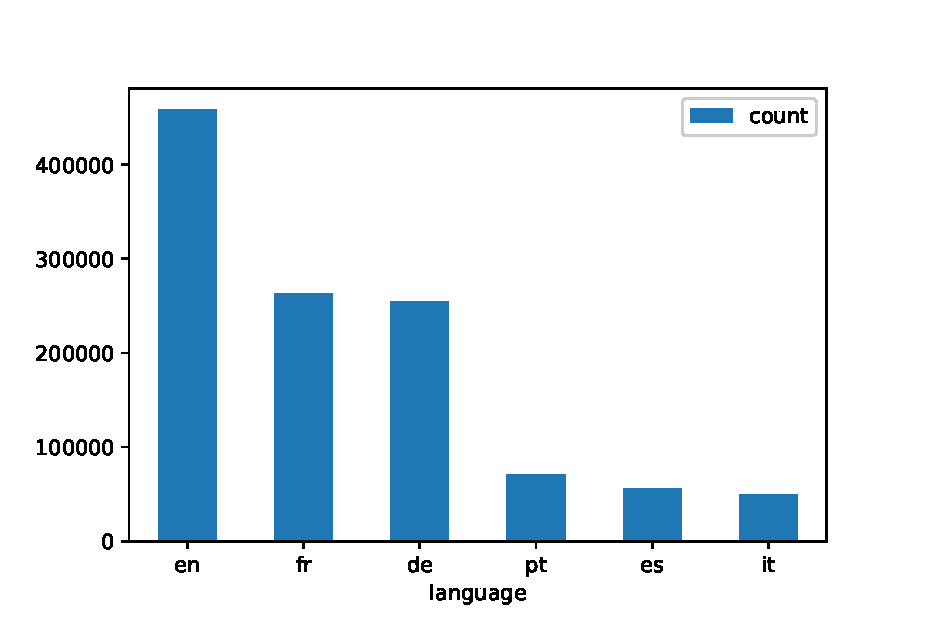
\includegraphics[width=0.45\textwidth]{images/swiss_counts16.eps}
  \caption{The number of tweets in the top5 languages only for 2016}
  \label{swiss_counts16}
\end{figure}

\subsection{Detecting political content}

TODO: Ramtin 

